\chapter{DUNE Project Management}
\label{ch:detectors-pm}

\section{Overview}

The international DUNE Project is responsible for managing all
contributions to the design, construction, installation and
commissioning of the DUNE near and far detectors.

As described in CDR \volintro, the DUNE Project is integrated within the
DUNE Collaboration.  The collaboration, in consultation with the
Fermilab director, is responsible for forming the international
project team.  The leaders of this team are the Technical Coordinator
(TC) and Resource Coordinator (RC), who are jointly appointed by the
DUNE Co-Spokespersons and the Fermilab Director.  The project receives
appropriate oversight from stakeholders including the Fermilab
Directorate and DOE.  A detailed description of the DUNE collaboration
structure along with its advisory and coordinating structures is
contained within CDR \volintro\ Chap. 4 "Organization and Management".

The DUNE Project is responsible for coordinating the work
packages assigned to each of the international partners contributing
to the effort.  These individual work packages, which are supported
through independent funding agencies, have internal management
structures that are responsible for satisfying the tracking and
reporting requirements of the supporting agencies.  However, the
entire project scope (including non-DOE partner contributions) will be
subject to the DOE critical decision process.

The international DUNE Project Office maintains a schedule for the
entire project and tracks individual contributions through detailed
sets of milestones embedded within the schedule.  It is also responsible
for ensuring that the interfaces between the different work package
deliverables are well defined and that all of these deliverables meet
safety and operational readiness requirements for installation at
Fermilab and the Sanford Underground Research Facility.  Project
Office members including the Project Manager are appointed by the TC.
The managers of the collaboration detector and prototyping
organizations report to the Project Manager and provide the required
interface between the DUNE project and the other members of the
collaboration contributing to these efforts.  As members of these
organizations, they participate in all discussions related to the
design, construction, installation and commissioning of individual
detector elements.  Managers have the primary responsibility for
implementing collaboration plans developed within their organizations.
 
Following this model, the DUNE-US project will have its own project
office and management structure.  All normal DOE project management
requirements will apply to the DUNE-US project.  In its role as host,
the DOE will provide financial support for both the international DUNE
Project Office and the DUNE-US Project Office. The DUNE TC, who acts
as Project Director in the context of the international DUNE project,
also serves as the DUNE-US Project Director.  However, each project
office will have its own project manager.  Other equivalent positions
within the project offices may be filled by the same individuals in
cases where the TC believes this sharing of resources to be most
efficient. Some project office staff may also overlap with the LBNF
project office as appropriate.

\section[Work Breakdown Structure (WBS)]{WBS}

The DUNE Project will manage all contributions to the design,
construction, installation and commissioning of the DUNE near and far
detectors through an international Work Breakdown Structure (WBS).
The WBS organizes the Project's tasks and deliverables into convenient
components and is used to organize the cost and schedule for the DUNE
project. The DUNE Project consists of two major subsystems: the Near Detector
(WBS 130.03), shown to WBS level 4 in Figure~\ref{fig:ND_WBS}, and the
Far Detector (WBS 130.05), shown to WBS level 3 in
Figure~\ref{fig:FD_WBS}.
\begin{cdrfigure}[Near detector WBS]{ND_WBS}{Near detector Work Breakdown Structure.}
\centering
\begin{center}
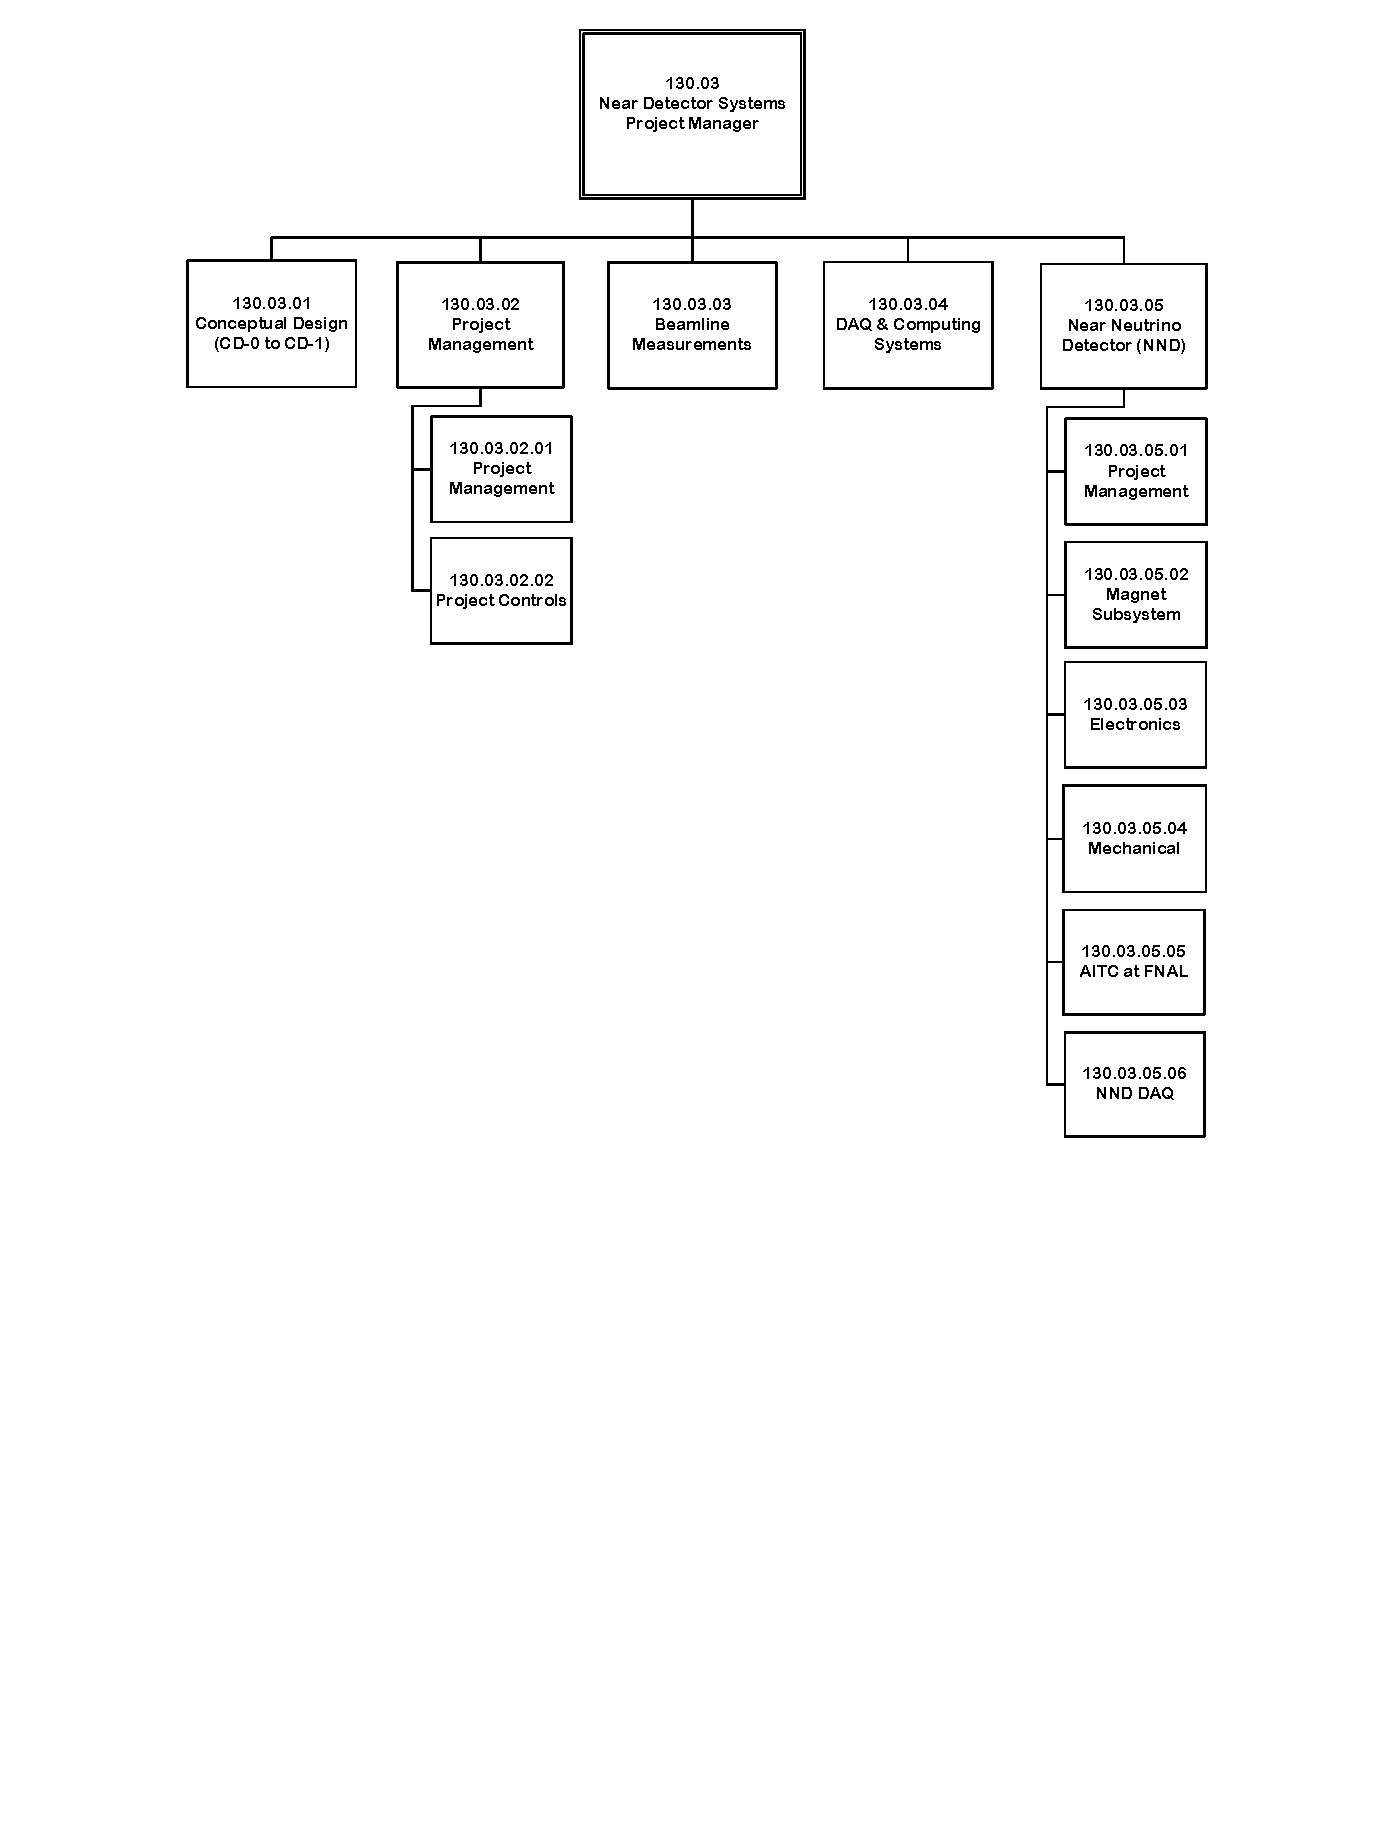
\includegraphics[width=0.85\textwidth]{ND_documents_nonames.pdf}
\end{center}
\end{cdrfigure}
\begin{cdrfigure}[Far detector WBS]{FD_WBS}{Far detector Work Breakdown Structure.}
\centering
\begin{center}
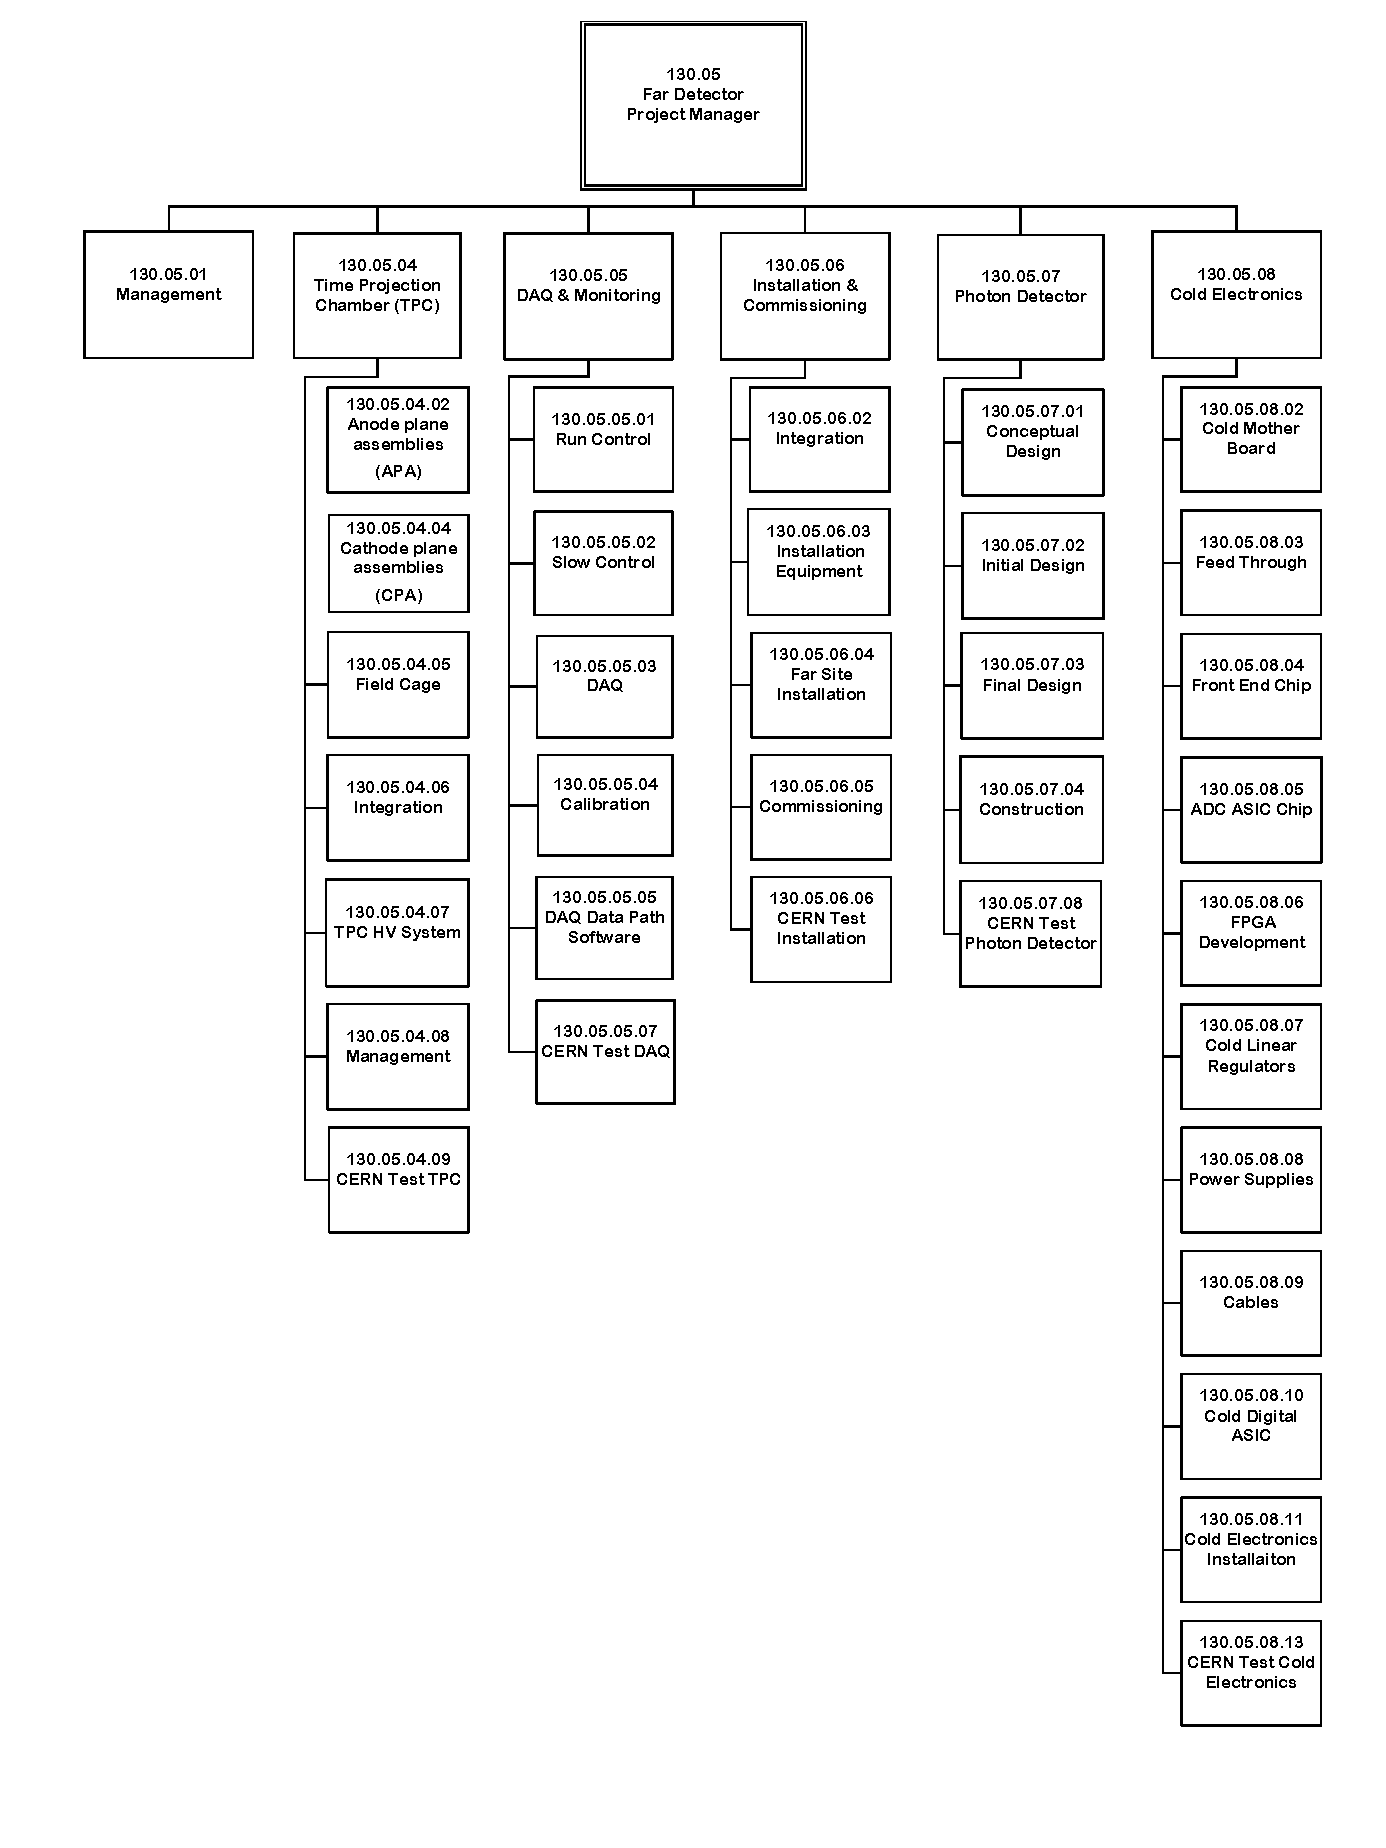
\includegraphics[width=0.9\textwidth]{FD_documents_nonames.pdf}
\end{center}
\end{cdrfigure}
The DUNE Project organization and structure will evolve as the project
becomes more fully internationalized.
